\documentclass[a4paper]{article}
\usepackage[warn]{mathtext}
\usepackage[utf8]{inputenc}
\usepackage[T2A]{fontenc}

\usepackage[english,russian]{babel}
\usepackage{multicol}
\usepackage{fancyhdr}
\usepackage{graphicx}
\usepackage{microtype}
\usepackage{wrapfig}
\usepackage{amsmath}
\usepackage{floatflt}
\usepackage{geometry} \geometry{verbose,a4paper,tmargin=2cm,bmargin=2cm,lmargin=1.5cm,rmargin=1.5cm}
\usepackage{float}
\usepackage{amssymb}
\usepackage{caption}
\usepackage{epsfig}
\usepackage{newunicodechar}

\begin{document}

\graphicspath{ {pictures/} }

\begin{titlepage}
	\centering
	\vspace{5cm}
    {\scshape\LARGE Московский физико-технический институт\par}
	\vspace{5cm}
	{\scshape\Large Вопрос по выбору \par}
    {\scshape\Large по курсу \par}
    {\scshape\Large <<Основы современной физики>> \par}
	\vspace{1cm}
    {\huge\bfseries  SIS переход \par}
	\vspace{1cm}
	\vfill
    \begin{flushright}
        {\large выполнил студент Б04-852 группы ФЭФМ}\par
        \vspace{0.3cm}
        {\LARGE Яромир Водзяновский}
    \end{flushright}
	\vfill
Долгопрудный, 2021
% Bottom of the page
\end{titlepage}

\pagestyle{fancy} 
\fancyhead[L]{SIS   $\sim  \hat(\, ^{\circ}  \omega  ^{\circ} \, \hat) \sim$}
% \fancyhead[L]{Закон Кюри-Вейса    $( *{^\circ}< >^{\circ}*)$}
\fancyhead[R]{Современная физика}
\fancyfoot[C]{ \noindent\rule{\textwidth}{0.4pt} \thepage }



\newpage

\section{Теория}

\subsection{Туннельные эффекты в сверхпроводниках}

\subsubsection{Принцип измерения}

Наиболее прямое измерение энергетической щели в сверзпроводниках может быть проведено с помощью туннелных экспериментов. \par 
\begin{itemize}
    \item На стеклянную пластинку, с подготовленными контактами наносится узкая полоска пленки первого металла.
    \item Далее эта полоска окисляется и покрывается слоем изолирующего окисла толщиной $\sim 10 $ ангсрем. 
    \item В поперечном направлении наносится узкая полоска пленки второго металла.
\end{itemize}

Место пересечения полосок ($S \sim 1\; мм^2$) и представляет собой туннелоный переход. 

\subsubsection{Туннельные характеристики}

\textbf{Cлучай $T = 0$.} Туннельный ток может возникнуть только тогда, когда к туннельному переходу будет приложено 
напряжение $V > (\Delta_1 - \Delta_2)/e$, как видно из рис.\ref{p1}. Электронная пара в $S_1$ разрывается, один электрон туннелирует в $S_2$ с 
выделением энергии $\geq \Delta_1$. Второй электрон, поглащая эту энергию позбуждается  в состояния спектра квазичастиц $S_1$.  

\begin{figure}[H]
    \begin{center}
        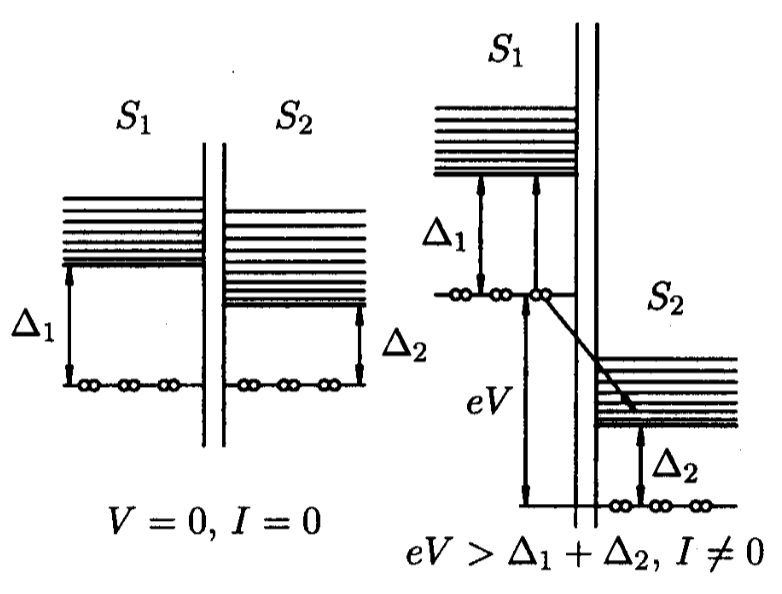
\includegraphics[scale = 0.5]{p1.png}
        \caption{Энергетические диаграммы для туннельного перехода $S_1IS_2, \; T = 0$}
        \label{p1}
    \end{center}
\end{figure}


\textbf{Cлучай $T \neq 0$.} Теперь в каждом из сверхпроводников имеется некое кол-во возбужденных одиночных электронов, равновесное кол-во которых определяется температурой. \par 

Диаграммы изображены на рис. \ref{p2}. \textit{Количеством точек указано количество возбуждений в данном состоянии.} Если $V = 0$, то не смотря на разные щели $\Delta_1 \neq \Delta_2$, кол-во возбуждений на противополжных уровнях в $S_1$ и $S_2$ будет одинаково.
Кол-во туннелирующих из $S_1$ в $S_2$ и обратно буде одинаковым, как в равновесном процессе $I = 0$. \par 

Если приложить небольшое напряжение $V$, то равновесие нарушиться и возникнет ток квазичастиц. Плотность стостояний квазичастиц в сверхпроводнике имеет особенность при $E = \Delta$. Если приложить к переходу разность потенциалов $V: \; eV = \Delta_1 - \Delta_2$, 
то друг против друга окажуться области с плотностью состояний $\rho = \infty$. Это вывовет \textbf{<<всплеск>>} туннельного тока, дальнейшее увеличение $V$ приведет к уменьшению тока, т.к уровни разойдутся. Отсюда, в точке $V = (\Delta_1 - \Delta_2)/e$ будет максимум тока. рис. \ref{p3}

\begin{figure}[H]
    \begin{center}
        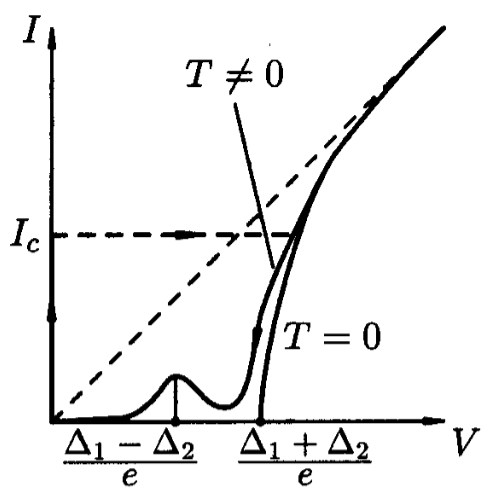
\includegraphics[scale = 0.5]{p3.png}
        \caption{Сверхпроводящие и квазичастичные ветви ВАХ у $S_1IS_2$ перехода для $T=0$ и $T \neq 0$.}
        \label{p3}
    \end{center}
\end{figure}

\begin{figure}[H]
    \begin{center}
        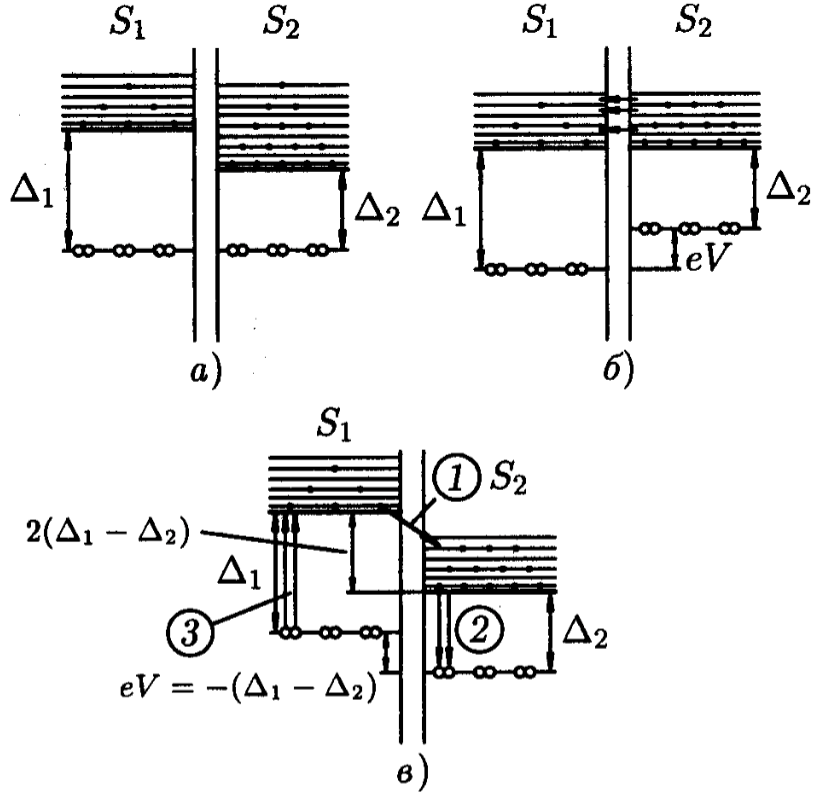
\includegraphics[scale = 0.5]{p2.png}
        \caption{Туннелирование между двумя сверхпроводниками при $T \neq 0$: \textbf{а)} $V=0$, концентрация возбуждений с одинаковой энергией $S_1, \; S_2$ одинакова, поэтому $I = 0$; \textbf{б)} $eV = \Delta_1-\Delta_2$, ток обусловлен переходом возбужденных частиц из $S_2$ в $S_1$; \textbf{в)} $eV = -(\Delta_1-\Delta_2)$, возбужденная частица переходит из $S_1$ в $S_2$ (1), объединившись с электронами в $S_2$, она образует пару и попадает на основной уровень (2), выделившейся энергии $2 \Delta_1$, достаточно для разрыва пары в $S_1$ (3). }
        \label{p2}
    \end{center}
\end{figure}




\subsection{Спектр элементарных возбуждений сверхпроводника}

\subsubsection{Энергетическая щель}

Возьмем пару состояний $(\mathbf{q}, -\mathbf{q})$ в импульсном пространстве сверхпроводника в основном состоянии. Эта пара вносит вклад в полную энергию $w_p$


\end{document}